\documentclass[10pt]{article} 
\usepackage[final]{graphicx} 
\usepackage{amsfonts} 
 \usepackage{amsmath}
\usepackage{tikz, flowchart}
\usetikzlibrary{arrows}
\topmargin-.5in 
\textwidth6.6in 
\textheight9in 
\oddsidemargin0in 
 
\def\ds{\displaystyle} 
\def\d{\partial} 

 
\begin{document} 

%
%
%
%
% PARTICIPANTS, MENTORS, AFFILIATIONS
%
%
%
%
%

\centerline{\large \bf Wine, Ebola and Terrorism}

\vspace{.1truein}

\def\thefootnote{\arabic{footnote}}
\begin{center}
  Hsuan-Wei Lee\footnote{Department of Mathematics, UNC Chapel Hill},
  Anzhelika Lyubenko\footnote{Department of Mathematical and Statistical Sciences, University of Colorado Denver},
  Yuhang Ma\footnote{Department of Operations Research and Information Engineering, Cornell University},
  Emily Meissen\footnote{Program of Applied Mathematics, University of Arizona},
  Daniela Velez-Rendon\footnote{Department of Bio-engineering, University of Illinois at Chicago},
    Nara Yoon\footnote{
Department of Mathematics, Applied Mathematics and Statistics, Case Western Reserve University}
\end{center}

%\vspace{.1truein}

\begin{center}
Mentors: John Peach \footnote{MIT Lincoln Labs}, Cammey Cole Manning\footnote{Meredith College},
Christian Gunning\footnote{NCSU}
\end{center}
%
%
%
%
% ABSTRACT
%
%
%
%
%

\vspace{.3truein}
\centerline{\bf Abstract}

We present a new model of Ebola outbreak in Liberia during 2014-2015. We approach the problem from both systematic and agent perspective and compare the results. We show that if the outbreak is not contained in the early stages and the individuals do not change their behavior as the virus prevails, between 60 and 80 percent of population get the disease. 

%
%
%
%
% INTRODUCTION
%
%
%
%
%
\section{Introduction}
Bacteria growth during wine making, spread of infectious diseases and recruitment to extremists organizations can be modeled in a similar way - either by exponential or logistic growth models. For the purposes of this paper we focus solely on modeling the spread of Ebola through Liberia throughout 2014 - 2015 outbreak. We chose to focus on Liberia because most of the data needed for the model was available in the literature. While the model allows one to consider other countries affected by the outbreak we did not calibrate the associated parameters. \\
%
%
%
Ebola was first discovered in 1976. Since then, there were 34 records of Ebola reported by the Center for Disease Control and Prevention. However, until 2014 all outbreaks had a reported number of deaths that did not exceed 500; 11 of them did not exceed 10 individuals and 15 records did not exceed 65 individuals \cite{CDCOutbreaks}.  The outbreak of 2014 is considered different. It took thousands of lives over the past two years and received an extensive media coverage.
%
%
%
The current outbreak may be different because it was the first time Ebola was contracted in the West Africa as opposed to Central Africa where it was first discovered. Early symptoms are flu-like: fever, headache, fatigue and joint pain. Diseases like HIV and Malaria, which are common to the region, have the same symptoms. As Ebola progresses, the infected experiences abdominal pain, diarrhea, vomiting and rashes. The virus is contracted through direct contact with bodily fluids and secretion: blood, saliva, urine, fecal matter. It can also be transmitted by physical contact with an object contaminated by such fluids. Once virus is contracted, the incubation period may last up to two weeks making intervention measures like tracking difficult \cite{CDCSympt}. 
%
%
%
\\A variety of cultural and economic factors have contributed to the spread of the disease: lack of medical centers in some regions and poor sensitization practices in such centers, distrust in the western medicine, poverty and traditional burial ceremony which includes physical contact with the diseased \cite{WHOReasons}. \\
%
%
%
One may look at the spread of the infectious diseases from two perspectives: system based and agent based. In the system based model the entire population is divided into compartments with a certain proportion of the population in each. As time progresses certain amount of people flow from one compartment into another. Naturally, such relationship is described either by a difference or a differential equation. One of the most well-known equation-based models involves three states: susceptible, infected, recovered. Such model is called an SIR model; each letter in the abbreviation represents one of the compartments in the population. This model has multiple modifications because various compartments can be added. In the case of Ebola, Lekone and Finkenstäd \cite{Lekone2006} consider a four compartment model, inserting an "Exposed" state between "Susceptible" and "Infected". A six-compartment model, presented by Legrand \cite{Legrand2007} and Rivers\cite{Rivers2014} differentiates between the modes of transition of the disease, i.e. a virus can be transmitted in the community, at hospitals and medical centers or at funerals.\\
In contrast to system based models, agent-based models are concerned with the behavior of a typical individual rather than the system as a whole. In such models every individual in the system is assigned certain characteristics, i.e. states. Individual's behavior is probabilistic at each unit of time and causes him either to transition to a different state or stay in his current state. Agent-based models for Ebola include Siettos et al \cite{Siettos2015} and Merler et al\cite{Merler2015}. A variety of models examine the effectiveness of intervention measures. Examples include contact tracing by Webb et al \cite{Webb2015} and travel restrictions by Poletto et al \cite{Poletto2014}.\\
In this paper we consider a seven compartment system based model as well as agent-based modification of the same model. We show \textbf{What did we show?!} \textbf{What about the model with spatial component?}\\
The rest of the paper is organized as follows. In section~\ref{sec:Model} we present our model. Section~\ref{sec:Data} describes our data and parameters. Section~\ref{sec:Results} discusses the results of numerical experiments. Section~\ref{sec:Summary} concludes.\\\\

It should be written as much as possible in non-technical terms, so that a
lay reader can understand the context and the contribution of the paper.

\begin{itemize}
\item Describe the problem you are trying to solve, the approach
you took, and summarize your contribution and results.

\item Review the history of this problem, and existing literature.

\item Give an outline of the rest of the paper.
\end{itemize}

\section{The Problem}
\begin{itemize}
\item Give a precise technical description of your problem. 

\item State and justify all your assumptions. 

\item Define notation. 

\item Describe your data, how you collected them, their properties,
and whether you did 
anything to them (removed noise, filled in missing data, 
applied normalizations).
\end{itemize}
%
%
%
%
% MODEL
%
%
%
%
%

\section{Model}\label{sec:Model}
%
%
%
We examine the problem from two perspectives. We present a system based model first and then discuss an agent-based modification of it. We then consider an agent-based model that incorporates agents' movement through space.  
%
% ASSUMPTIONS
%
\subsection{Assumptions}
\begin{itemize}
\item We consider a model of Ebola Outbreak with parameters calibrated for Liberia.
\item We consider two time periods. The first one starts with the announcement of Ebola outbreak in March 2014 and ends the day of the International Intervention in September 2014. The second period covers the time from the International Intervention to present.
\item We ignore all the possible births and deaths occurred due to reasons other that Ebola during the chosen time. 
\item Each individual who dies because of Ebola has a funeral.
\end{itemize}
\subsection{Compartment-State Definition}
\begin{description}
\item[S]- Susceptible. Individuals who have not contracted the disease and have no immunity to it. 
\item [E] - Exposed. Individuals who have come in contact with the Ebola patient and have contracted the disease but do not yet exhibit sever symptoms and thus, are considered not infectious.
\item [I] - Infected. Individuals who experience severe symptoms of Ebola and are contagious.
\item [H] - Hospitalized. Individuals who are infectious and are in the hospital because they are experiencing severe symptoms of Ebola.
\item[F] - Funeral. Diseased but still contagious victims of Ebola. 
\item[D] - Dead. Individuals who died because of Ebola, were buried and are currently under ground. They are considered not to be contagious.
\item [R] - Recovered. Individuals who had Ebola,survived and now are immune to the disease.
\end{description}
%
% SYSTEM BASED
%
\subsection{System Based}
Based on the compartmental model and parameters published by Rivers et al.\cite{Rivers2014} in October 2014, it was modeled a similar approach in Insight Maker.  This particular model, divides the population into six different compartments; the Susceptible persons (S) could turn into Exposed (E), if they were in contact with an infections individual, initiating a trantition to the Infectious (I) state after the incubation period of the disease, subsequently, acquiring the capacity of infecting others. A percentage of the I class individuals may be Hospitalized (H). There are two possible outcomes for the untreated individuals in I and the treated patients in H, individuals may die, with a probability of infecting other people during the resultant Funeral (F), before the virus is removed from the individual (R), or the patients may recover, at this stage, it can be cosidered equivalently removed. However, for the present study was considered seven compartments in order to distinguish between the recovered (R) patients and the deceased (D) individuals. Figure ~\ref{fig:compartment} depicts the implemented compartment model. \\

\begin{figure}[h!]
  \centering
  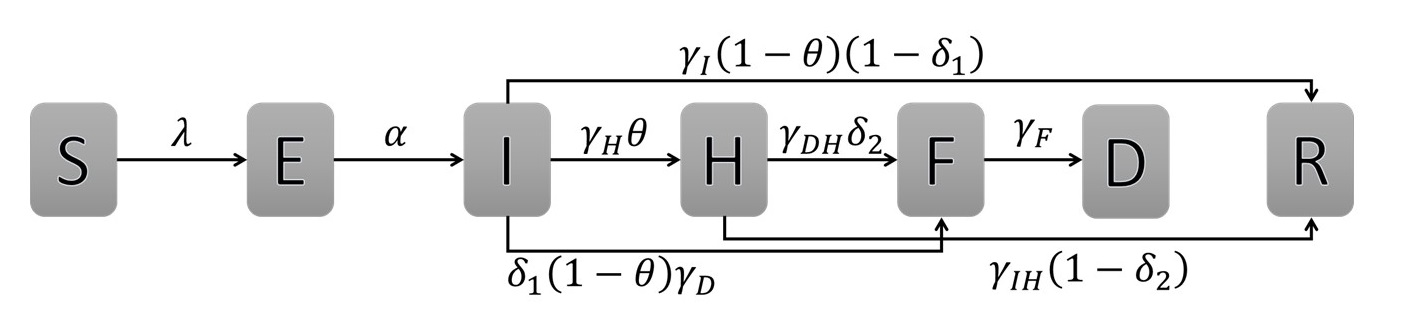
\includegraphics[width=0.7\textwidth]{compartment}
  \caption{Compartment Model of the Ebola Epidemic in Liberia and Sierra Leone \newline  Being S: Susceptible, E: Exposed, I: Infectious, H: Hospitalized, F: Funeral,  R: Recovered and D: Dead. All the possible flows are specified by the arrows and the parameters that direct them. Note that $\lambda = \beta_{I}I+\beta_{H}H+\beta_{F}F $, being a combination of all the $\beta$ transmission terms shown in Table~\ref{tab:parameters}} 
\label{fig:compartment} 
\end{figure}

 
The governing equations of the system described above are the following:
\begin{align*} 
\frac{dS}{dt} &= - \frac{\beta_{I}SI+\beta_{H}SH+\beta_{F}SF}{N}\\
\frac{dE}{dt} &=  \frac{\beta_{I}SI+\beta_{H}SH+\beta_{F}SF}{N}-\alpha E\\
\frac{dI}{dt} &=  \alpha E - [\gamma_{H}\theta + \gamma_{I}(1-\theta)(1-\delta_{1})+\gamma_{D}(1-\theta)\delta_{1}]I\\
\frac{dH}{dt} &= \gamma_{H}\theta I - [\gamma_{DH}\delta_{2}+\gamma_{IH}(1-\delta_{2})]H\\
\frac{dF}{dt} &= \gamma_{D}(1-\theta) \delta_{1} I + \gamma_{DH}\delta_{2} H-\gamma_{F} F\\
\frac{dR}{dt} &= \gamma_{I}(1-\theta)(1- \delta_{1}) I + \gamma_{IH}(1-\delta_{2}) H-\gamma_{F} F
\end{align*}
where each of the parameters are defined on Table \ref{tab:parameters}


\begin{table}[ht]
\caption{Model Parameters for Ebola Epidemic in Liberia Before  and After the International Intervention} % title of Table
\centering % used for centering table
\begin{tabular}{c c c } 
\hline\hline %inserts double horizontal lines
Parameter & Liberia Before Intervention  & Liberia After Intervention \\ [0.5ex] 
 & (Mar/14 to Sept/14) &  (Sept/14 to Jul/15) \\ [0.5ex] % inserts table
% inserts table
%heading
\hline % inserts single horizontal line
Contact Rate, Community  ($\beta_{I}$) & 0.148 & 0.0446  \\ 
Contact Rate, Hospital  ($\beta_{H}$) & 0.235 & 0.0877  \\
Contact Rate, Funeral  ($\beta_{F}$) & 0.465 & 0.283 \\
Incubation Period (${1}/{\alpha}$) & 11 days & 11 days  \\
Time until Hospitalization (${1}/{\gamma_{H}}$) & 4.49 days & 4.63 days  \\
Time froml Hospitalization to Death (${1}/{\gamma_{DH}}$) & 3.51 days & 3.51 days  \\ 
Duration of Traditional Funeral (${1}/{\gamma_{F}}$) & 2.00 days & 2.00 days  \\
Duration of Infection (${1}/{\gamma_{I}}$) & 10.00 days & 10.00 days  \\
Time from Infection to Death (${1}/{\gamma_{D}}$) & 8.00 days & 8.00 days  \\
Time from Hospitalization to Recovery (${1}/{\gamma_{IH}}$) & 5.51 days & 5.51 days  \\
Probablity a Case is Hospitalized ($\theta$) & 0.248 & 0.233 \\
Case Fatality Rate, Unhospitalized ($\delta_{1}$) & 0.500  & 0.500  \\
Case Fatality Rate, Hospitalized ($\delta_{2}$) & 0.500 & 0.500 \\ [1ex] 
\hline 
\end{tabular}
\label{tab:parameters}
\end{table}

%\begin{figure}
%\begin{tikzpicture}[->,>=stealth',shorten >=1pt,auto,node distance=3cm,
%  thick,main node/.style={circle,fill=blue!20,draw,font=\sffamily\Large\bfseries}]
%
%  \node[main node] (1) {S};
%  \node[main node] (2) [right of=1] {E};
%  \node[main node] (3) [right of=2] {I};
%  \node[main node] (4) [right of=3] {R};
%    \node[main node] (5) [below left of=3] {D};
%      \node[main node] (6) [below right of=3] {F};
%        \node[main node] (7) [right of=6] {H};
%
%  \path[every node/.style={font=\sffamily\small}]
%    (1)
%        edge node {$f_{SE}$} (2)
% 
%    (2) edge node {$f_{EI}$} (3)
%        
%    (3) 
%       edge node {$f_{IR}$} (4)
%       edge node[left] {$f_{IF}$} (6)
%       edge node {$f_{IH}$} (7)
%  
%    (4)
%       
%(6) edge node{$f_{FD}$} (5) 
%
%(7) edge node[right]{$f_{HR}$} (4) 
%
%  (7) edge node{$f_{HF}$} (6)      
%
%        ;
%        
%\end{tikzpicture}
%\caption{Model}
%\label{SM}
%\end{figure}
%
% AGENT BASED
%
\subsection{Agent Based} 
The next model we consider is an agent-based model. Each individual in the population can be in either of 7 states discussed above: susceptible, exposed, infected, hospitalized, funeral, recovered or dead. The flow between two states is a  probability of transition from one state to another for a typical individual. We represent our model in Figure~\ref{ABM}. In each time step a typical individual who is susceptible to contracting a virus can either transition to exposed state with probability $p_{SE}$ or stay susceptible with probability $p_{SS}$. An individuas in the exposed state transitions to infected with probability $p_{EI}$ and stays exposed with probability $p_{EE}$. An individual who is infected can stay infected, recover, go to a hospital or die and transition to funeral state with probabilities $p_{II},\, p_{IR},\, p_{IH}$ and $p_{IF}$ respectively. Recovery is considered a terminal state so individuals in this state stay in it for the remaining duration of the simulation. Hospitalized individuals may stay hospitalized, transition to recovered or funeral with probabilities $p_{HH}, \, p_{HR}$ and $p_{HF}$. We assume that the individual who dies from Ebola remains infectious through the duration of the entire burial ceremony and no precautions are taken against disease transmission. Safely buried individuals are considered dead and noninfectious and remain in this state for the remaining time of the simulation.  

%  \begin{tikzpicture}[node distance=2cm, font=\tiny]
%        \node [draw, terminal]  (start) at (0,0) {Start};
%        \node [draw, predproc, right of= start] (acquire)(write) {Acquire Image};
%
%%% paths
%    \draw[->](work) -- node[above]{yes}(end);
%    \end{tikzpicture}
\begin{figure}[h!]
\begin{center}
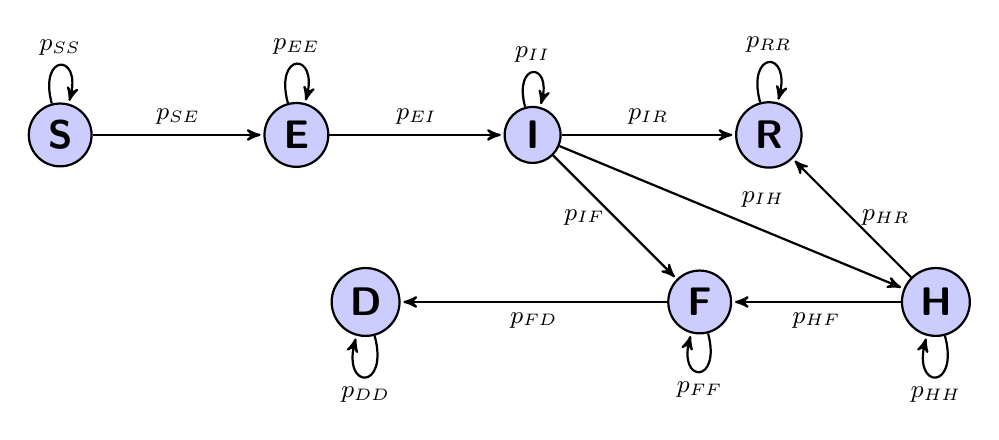
\begin{tikzpicture}[->,>=stealth',shorten >=1pt,auto,node distance=3cm,
  thick,main node/.style={circle,fill=blue!20,draw,font=\sffamily\Large\bfseries}]

  \node[main node] (1) {S};
  \node[main node] (2) [right of=1] {E};
  \node[main node] (3) [right of=2] {I};
  \node[main node] (4) [right of=3] {R};
    \node[main node] (5) [below left of=3] {D};
      \node[main node] (6) [below right of=3] {F};
        \node[main node] (7) [right of=6] {H};

  \path[every node/.style={font=\sffamily\small}]
    (1)
        edge node {$p_{SE}$} (2)
        edge [loop above] node {$p_{SS}$} (1)
    (2) 
        edge node {$p_{EI}$} (3)
         edge [loop above] node {$p_{EE}$} (2)
      
    (3) 
       edge node {$p_{IR}$} (4)
       edge node[left] {$p_{IF}$} (6)
       edge node {$p_{IH}$} (7)
        edge [loop above] node {$p_{II}$} (3)
    (4)
         edge [loop above] node {$p_{RR}$} (4)
       
(6) edge node{$p_{FD}$} (5) 
edge [loop below] node {$p_{FF}$} (6)     
(7) edge node[right]{$p_{HR}$} (4) 
edge [loop below] node {$p_{HH}$} (7)
  (7) edge node{$p_{HF}$} (6)      
 (5) edge [loop below] node {$p_{DD}$} (5)
        ;
        
\end{tikzpicture}
\end{center}
\caption{Spread of the disease: Agent-based model. Each node represents a typical individual's state. An individual can transition to a state to which he is connected by a directed arc with a probability specified on an arc}
\label{ABM}
\end{figure}
Let

\begin{itemize}
\item[]$t_{IP}$ be the incubation period, i.e. time during which the individual has the virus in his body but does not yet show severe symptoms
\item[] $t_{ID}$ infection duration time ater the onset of severe symptoms
\item[] $t_{H}$ time to hospitalization after manifistation of severe symptoms
\item[] $t_{IF}$ time from the onset of severe symptoms to funeral
\item[] $t_{HF}$ time from patient's arrival at the hospital to fueral
\item[] $t_{HR}$ time from patient's arrival at the hospital to recovery
\item[] $t_{DF}$ duration of traditional funeral
\item[] $N$  total number of individuals in a population
\item[] $N_{I}$  total number of individuals in the infected state
\item[] $N_{H}$  total number of individuals in the hospitalized state
\item[] $N_{F}$  total number of individuals in the funeral state
\item[] $\beta_{I}$ rate at which the disease spreads during an interaction with an infected person
\item[] $\beta_{H}$ rate at which the disease spreads during an interaction with a hospitalized person
\item[] $\beta_{F}$ rate at which the disease spreads during an interaction with a person who is in the funeral state
\end{itemize}
We define the individual's probability ofl transition for each state as

\begin{subequations}
\begin{alignat}{1}
&p_{SE}=\beta_I\cdot \frac{N_{I}}{N}+\beta_H\cdot \frac{N_{H}}{N}+\beta_F\cdot\frac{ N_F}{N}\\
&p_{SS}=1-p_{SE}\\
&p_{EE}=1-\frac{1}{t_{IP}}\\
&p_{EI}=\frac{1}{t_{IP}}\\
&p_{II}=\frac{1}{t_{ID}}\\
&p_{IH}=\frac{1}{t_{H}}\\
&p_{IF}= \frac{1}{t_{IF}}\\
&p_{IR}=1-p_{II}-p_{IH}-p_{IF}\\
&p_{HF}=\frac{1}{t_{HF}}\\
&p_{HR}=\frac{1}{t_{HR}}\\
&p_{HH}=1-p_{HF}-p_{HR}\\
&p_{FF}=\frac{1}{t_{DF}}\\
&p_{FD}=1-p_{FF}\\
&p_{RR}=1\\
&p_{DD}=1
\end{alignat}
\end{subequations}
\subsection{Strategy}
In order to propose a more accurate model and compare the results among different programming  languages, the compartment flow model of the Ebola Epidemic in West Africa, 2014, was modeled with a System Dynamics (SD) and Agent Based Model (ABM) approaches.  Insight Maker and Mathematica was utilized  for the SD, and Insight Maker and Python for the ABM.

\subsection{Factors Considered}
There are several factors to take into account when analyzing how a virus may spread in a community. First of all the customs and beliefs of a society play an important role, it implies how the individuals interact among themselves, how often they visit their relatives or friends, the amount of travel to other villages, cities or countries to work or buy supplies, as well as the mode of transport.\\
Having information about the local government and the wealth of the region, would help to determine the capacity of response when facing an epidemic; including the quantity and quality of hospitals and their capacity, as well as the amount of healthcare workers and their expertise.\\
In the moment of a virus outbreak, goverments from other countries may intervent to help to control the disease, possibly decreasing the number of infected people and increased the number of recovered patients, by educating individuals about the virus, the ways of transmission and handling of the deceased family. \\
Characteristics of the virus itself are also important, having an estimate of the incubation period, the rate of recovery, the time it remains in the deceased would help to predict the behavior of the virus.\\

\subsection{Software}
\begin{itemize}
\item Insight Maker: SD and ABM
\item Mathematica: SD
\item Python: ABM

\end{itemize}
We used InsightMaker platform to prototype our model and simulate stepping forward through time. More details about the platform and its functionality can be found in Fortmann-Roe's review \cite{FortmannRoe}. The platform uses fourth order Runge-Kutta differential equation solver for the system dynamics model and  first order Euler approximation for the Agent-Based model.

%
%
%
%
% DATA
%
%
%
%
%
\section{Data}\label{sec:Data}
We used data reported by World Health Organization recorded by the Center for Disease Control and Prevention \cite{CDCData} to calibrate the parameters of the model. 
%The United Nation reports that the last Census for the countries of Guinea, Sierra Leone, Liberia and Nigeria  was conducted in 2014, 2004, 2008 and 2006 respectively. Due to the need for estimating more current demographic data, we used CIA Factbook estimates. 

\section{Computational Experiments}
\subsection{Compartment Model: System Dynamics}
\subsection{Agent-Based Model}
We consider a population of size \textbf{100} with \textbf{99} individuals starting in a susceptible state and \textbf{1} individual in the exposed state. Numeric probabilities of an individual transitioning from each state are recorded in Table \textbf{CREATE A TABLE}. We simulate \textbf{176} days of disease progression without intervention and \textbf{306} days of post intervention disease progression. We repeat the process \textbf{100} times and record the average outcome.  

\subsection{Compartment Model: Agent Dynamics}
The agent-based model created in Insight Maker also used the data from Rivers et al. with the same states and parameter names as the System Dynamics model. The transitions between the states are described as:\\

\begin{table}[ht]
\begin{center}
\begin{tabular}{c | l | l}
{\bf Transition} & {\bf Type } & {\bf Value}\\\hline
$S\rightarrow E$ & Probability & $\min(1,\xi_5\beta_{fam}+\xi_{100}\beta_{com}+\xi_{10}\beta_F)$\\
$E\rightarrow I$ & Timeout & $1/\alpha$\\
$I\rightarrow H$ & Probability & $\theta\gamma_H$\\
$I\rightarrow F$ & Probability & $(1-\theta)\delta_1\gamma_D$\\
$I\rightarrow R$ & Probability & $(1-\theta)(1-\delta_{1})\gamma_I$\\
$F\rightarrow R$ & Timeout & ${1}/{\gamma_{F}}$\\
$H\rightarrow R$ & Timeout & $\delta_{2}/{\gamma_{DH}} + (1-\delta_{2})/{\gamma_{IH}}$\\
\end{tabular}
\end{center}
\end{table}
\noindent where $\xi_{i}$ is the number of infected people within the individual's $i$ closest neighbors, $\beta_{fam}$ is the family contact rate, and $\beta_{com}$ is the community contact rate (maybe same?). The probability of contracting Ebola depends on the number of infected people within the individual's family or neighbors, and funerals are assumed to be attended by the deceased's 10 nearest neighbors.

\begin{figure}
\caption{The agent-based Insight Maker model.}
\end{figure}

\begin{figure}
\caption{A simulation of the agent-based Insight Maker model with $\beta_{fam}=0.4$ and $\beta_{com}=0.01$.}
\end{figure}

\subsubsection{Insight Maker}

\subsubsection{Mathematica}
vxzv

\subsection{Compartment Model: Agent Based Model}


\subsubsection{Insight Maker}
czc

\subsubsection{Python}
zcx


Give enough details so that readers can duplicate your experiments.

\begin{itemize}
\item Describe the precise purpose of the experiments, and what they 
are supposed to show.

\item Describe and justify your test data, and any assumptions you made to 
simplify the problem.

\item Describe the software you used, and the 
parameter values you selected.

\item 
For every figure, describe the meaning and units of the coordinate axes, 
and what is being plotted.

\item Describe the conclusions you can draw from your experiments
\end{itemize}
%
%
%
%
% RESULTS AND DISCUSSION
%
%
%
%
%
\section{Results}\label{sec:Results}
%
%
%
%
% SUMMARY AND FUTURE WORK
%
%
%
%
%


\section{Summary and Future Work}\label{sec:Summary}
\begin{itemize}
\item Briefly summarize your contributions, and their possible
impact on the field (but don't just repeat the abstract or introduction).
\item Identify the limitations of your approach.
\item Suggest improvements for future work.
\item Outline open problems.
\end{itemize}
\bibliography{references}
\bibliographystyle{plain}

%
%
%
%
% APPENDIX (CODES)
%
%
%
%
%
\newpage
\appendix
\section{\\MATLAB Code for Agent-Based Model} \label{App:AppendixA}

\begin{verbatim}
clear;
clc;

SimulationNUM = 100;
population = 200;
timestep = 500;

beta_I = 0.16;
beta_H = 0.062;
beta_F = 0.489;
Incubation = 12;
InfDur = 15;
TimeToHosp = 3.24;
TimeInfDeath = 13.31;
TimeHospDeath = 10.07;
TimeHospRec = 15.88;
DurFun = 2.01;

% Transition matrix [S E I H F R D]
Tran = [0.5 0.5 0 0 0 0 0; 
      0 1-1/Incubation 1/Incubation 0 0 0 0
      0 0 1/InfDur 1/TimeToHosp 1/TimeInfDeath 1-1/InfDur-1/TimeToHosp-1/TimeInfDeath 0; 
      0 0 0 1-1/TimeHospDeath-1/TimeHospRec 1/TimeHospDeath 1/TimeHospRec 0; 
      0 0 0 0 1/DurFun 0 1-1/DurFun; 
      0 0 0 0 0 1 0; 
      0 0 0 0 0 0 1];

final_S = zeros(1,SimulationNUM);
final_R = zeros(1,SimulationNUM);
final_D = zeros(1,SimulationNUM);


for s = 1:SimulationNUM

people = [1 zeros(1,population-1)]; % initialization 

c0=zeros(1,timestep);
c1=zeros(1,timestep);
c2=zeros(1,timestep);
c3=zeros(1,timestep);
c4=zeros(1,timestep);
c5=zeros(1,timestep);
c6=zeros(1,timestep);

a0 = sum(people == 0); %compute how many people are 0 at timestep 1
a1 = sum(people == 1); %compute how many people are 1 at timestep 1
a2 = sum(people == 2); %compute how many people are 2 at timestep 1
a3 = sum(people == 3); %compute how many people are 3 at timestep 1
a4 = sum(people == 4); %compute how many people are 4 at timestep 1
a5 = sum(people == 5); %compute how many people are 5 at timestep 1
a6 = sum(people == 6); %compute how many people are 6 at timestep 1

c0(1)=a0;
c1(1)=a1;
c2(1)=a2;
c3(1)=a3;
c4(1)=a4;
c5(1)=a5;
c6(1)=a6;

SroE = zeros(1,timestep);

for t=2:timestep

d0=0; %change of amount
d1=0;
d2=0;
d3=0;
d4=0;
d5=0;
d6=0;    
    
StoE(t) = (beta_I*c2(t-1)+beta_H*c3(t-1)+beta_F*c4(t-1))/population;

for i=1:population
    
r=rand(1,population); %comparison vector
    
    
    if people(i)==0     % S goes to S or E
        if r(i)<=StoE(t)
            people(i)=1;
            d1=d1+1;
            d0=d0-1;
        end
    elseif people(i)==1 % E goes to E or I 
        if r(i)<=Tran(2,3)
            people(i)=2;
            d2=d2+1;
            d1=d1-1;
        end
    elseif people(i)==2 % I goes to I, H, F or R
        if r(i)<=Tran(3,4)
            people(i)=3;
            d3=d3+1;
            d2=d2-1;
        elseif Tran(3,4)<r(i)<=Tran(3,4)+Tran(3,5)
            people(i)=4;
            d4=d4+1;
            d2=d2-1;
        elseif Tran(3,4)+Tran(3,5)<r(i)<=Tran(3,4)+Tran(3,5)+Tran(3,6)
            people(i)=5;
            d5=d5+1;
            d2=d2-1;
        end
    elseif people(i)==3 % H goes to H, F or R
        if r(i)<=Tran(4,5)
            people(i)=4;
            d4=d4+1;
            d3=d3-1;
        elseif Tran(4,5)<r(i)<=Tran(4,5)+Tran(4,6) 
            people(i)=5;
            d5=d5+1;
            d3=d3-1;
        end
    elseif people(i)==4 % F goes to F or D
        if r(i)<=Tran(5,7)
            people(i)=6;
            d6=d6+1;
            d4=d4-1;
        end
        
    end  
    
    c0(1,t) = c0(1,t-1) + d0;
    c1(1,t) = c1(1,t-1) + d1;
    c2(1,t) = c2(1,t-1) + d2;
    c3(1,t) = c3(1,t-1) + d3;
    c4(1,t) = c4(1,t-1) + d4;
    c5(1,t) = c5(1,t-1) + d5;
    c6(1,t) = c6(1,t-1) + d6;
    
end
people;
end

people;
SUM_OF_PEOPLE = sum(c0(1,timestep)+c1(1,timestep)+c2(1,timestep)+c3(1,timestep)
              +c4(1,timestep)+c5(1,timestep)+c6(1,timestep));


 figure
 subplot(4,2,[1,2]);
 plot(c0/population,'LineWidth',2)
 axis([1 timestep 0 1])
 title('Proportion of S State')
 
 subplot(4,2,3);
 plot(c1/population,'LineWidth',2)
 axis([1 timestep 0 1])
 title('Proportion of E State')
 
 subplot(4,2,4);
 plot(c2/population,'LineWidth',2)
 axis([1 timestep 0 1])
 title('Proportion of I State')
 
 subplot(4,2,5);
 plot(c3/population,'LineWidth',2)
 axis([1 timestep 0 1])
 title('Proportion of H State')
 
 subplot(4,2,6);
 plot(c4/population,'LineWidth',2)
 axis([1 timestep 0 1])
 title('Proportion of F State')
 
 subplot(4,2,7);
 plot(c5/population,'LineWidth',2)
 axis([1 timestep 0 1])
 title('Proportion of R State')
 
 subplot(4,2,8);
 plot(c6/population,'LineWidth',2)
 axis([1 timestep 0 1])
 title('Proportion of D State')


final_S(s) = c0(timestep)/population;
final_R(s) = c5(timestep)/population;
final_D(s) = c6(timestep)/population;

end

final_S
final_R
final_D

% to compute the mean
% A = 1 - final_S
% for i = 1:100
%     if A(i) < 0.1
%         A(i)=0
%     end
% end
% A(A==0) = [];
% mean(A)


\end{verbatim}

\end{document}

